% !TEX TS-program = pdflatex
% !TEX encoding = UTF-8 Unicode

% This is a simple template for a LaTeX document using the "article" class.
% See "book", "report", "letter" for other types of document.

\documentclass[20pt]{article} % use larger type; default would be 10pt

\usepackage[utf8]{inputenc} % set input encoding (not needed with XeLaTeX)

%%% Examples of Article customizations
% These packages are optional, depending whether you want the features they provide.
% See the LaTeX Companion or other references for full information.

%%% PAGE DIMENSIONS
\usepackage{geometry} % to change the page dimensions
\geometry{a4paper} % or letterpaper (US) or a5paper or....
% \geometry{margin=2in} % for example, change the margins to 2 inches all round
% \geometry{landscape} % set up the page for landscape
%   read geometry.pdf for detailed page layout information

\usepackage{graphicx} % support the \includegraphics command and options

% \usepackage[parfill]{parskip} % Activate to begin paragraphs with an empty line rather than an indent

%%% PACKAGES
\usepackage{booktabs} % for much better looking tables
\usepackage{array} % for better arrays (eg matrices) in maths
\usepackage{paralist} % very flexible & customisable lists (eg. enumerate/itemize, etc.)
\usepackage{verbatim} % adds environment for commenting out blocks of text & for better verbatim
%\usepackage{subfig} % make it possible to include more than one captioned figure/table in a single float
\usepackage{mathtools}
\usepackage{graphicx} % supports images in latex
% These packages are all incorporated in the memoir class to one degree or another...

\usepackage{graphicx}
\usepackage{subcaption}

%%% Other stuff
\DeclarePairedDelimiter\ceil{\lceil}{\rceil}
\DeclarePairedDelimiter\floor{\lfloor}{\rfloor}

%%% HEADERS & FOOTERS
\usepackage{fancyhdr} % This should be set AFTER setting up the page geometry
\pagestyle{fancy} % options: empty , plain , fancy
\renewcommand{\headrulewidth}{0pt} % customise the layout...
\lhead{}\chead{}\rhead{}
\lfoot{}\cfoot{\thepage}\rfoot{}

%%% SECTION TITLE APPEARANCE
\usepackage{sectsty}
\allsectionsfont{\sffamily\mdseries\upshape} % (See the fntguide.pdf for font help)
% (This matches ConTeXt defaults)

%%% ToC (table of contents) APPEARANCE
\usepackage[nottoc,notlof,notlot]{tocbibind} % Put the bibliography in the ToC
\usepackage[titles,subfigure]{tocloft} % Alter the style of the Table of Contents
\renewcommand{\cftsecfont}{\rmfamily\mdseries\upshape}
\renewcommand{\cftsecpagefont}{\rmfamily\mdseries\upshape} % No bold!

%%% graphics path


%%% END Article customizations

%%% nice things to keep around

% \noindent\rule{2cm}{0.4pt} 
%%% puts a small horizontal line

% \mathcal{O} 
%%% big O notation

%%% The "real" document content comes below...

\title{Formal Languages Homework 1}
\author{Liam Dillingham}
%\date{} % Activate to display a given date or no date (if empty),
         % otherwise the current date is printed 

\begin{document}
\maketitle

\section{Problem 2.2.4}
Give DFA's accepting the following languages over the alphabet $\{0,1\}$:
\subsection{a). The set of all strings ending in $00$.}
\begin{figure}[!htb]
\center{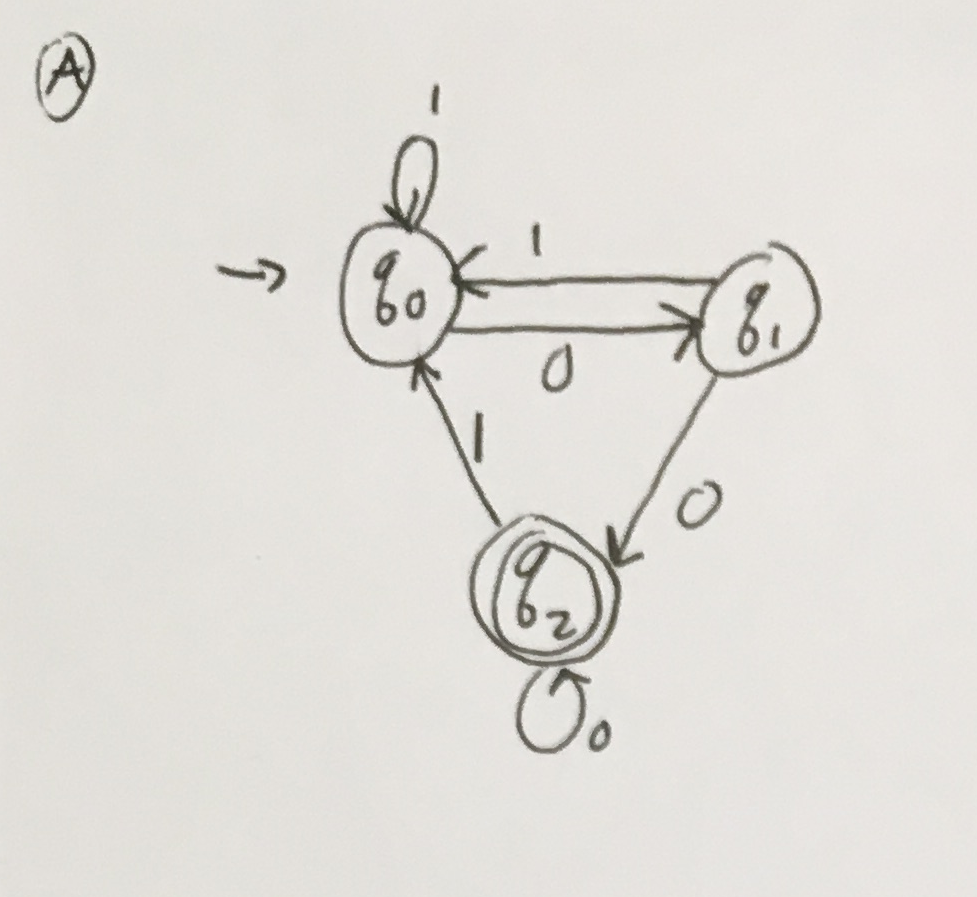
\includegraphics[width=\textwidth]{./figures/H1a.png}}

\end{figure}
\subsection{b). the set of all strings with three consecutive 0's (not necessarily at the end)}

\subsection{c). The set of strings with 011 as a substring}

\section{Problem 2.2.5}
Give DFA's accepting the following lagnuages over the alphabet $\{0,1\}$.
\subsection{a). The set of all strings such that each block fo five consecutive symbols contains at least two 0's.}

\subsection{b). The set of all string whose tenth symbol from the right end is a 1.}

\subsection{c). The set of strings that either begin or end (or both) with $01$.}

\subsection{d). The set of strings such that the nubmer of 0's is divisible by five, and the number of 1's is divisible by 3.}

\section{Problem 2.2.7}
Let $A$ be a DFA and $q$ a particular state of $A$, such that $\delta(q,a)=q$ for all input symbols $a$. 
Show by induction on the length of the input that for all input strings $w$, $\hat{\delta}(q,w)=q$.

\section{Problem 2.2.8}
Let $A$ be a DFA and $a$ a particular input symbol of $A$, such that for all states $q$ of $A$ we have $\delta(q,a)=q$.

\subsection{a). Show by induction on $n$ that for all $n\geq0$, $\delta(q,a^{n})=q$, where $a^{n}$ is the string consisting of $n$ $a$'s.}

\subsection{b). Show that if $x$ is a nonempty string in $L(A)$, then for all $k>0$, $x^{k}$ (i.e., $x$ written $k$ times is also in $L(A)$.)}

\end{document}
